\documentclass[12pt,a4paper]{article}%
%Options -- Point size:  10pt (default), 11pt, 12pt
%        -- Paper size:  letterpaper (default), a4paper, a5paper, b5paper
%                        legalpaper, executivepaper
%        -- Orientation  (portrait is the default)
%                        landscape
%        -- Print size:  oneside (default), twoside
%        -- Quality      final(default), draft
%        -- Title page   notitlepage, titlepage(default)
%        -- Columns      onecolumn(default), twocolumn
%        -- Equation numbering (equation numbers on the right is the default)
%                        leqno
%        -- Displayed equations (centered is the default)
%                        fleqn (equations start at the same distance from the right side)
%        -- Open bibliography style (closed is the default)
%                        openbib
% For instance the command
%           \documentclass[a4paper,12pt,leqno]{article}
% ensures that the paper size is a4, the fonts are typeset at the size 12p
% and the equation numbers are on the left side

% Tabelas
\usepackage{multirow}

% Símbolos Matemáticos
\usepackage{amsmath}
\usepackage{amsfonts}
\usepackage{amssymb}
\usepackage{bm}
\usepackage{commath}
\usepackage{steinmetz}
\usepackage{mathrsfs}

% Figuras
\usepackage{graphicx}
\usepackage{wrapfig}
\usepackage{float}
\usepackage{subfigure}
\graphicspath{ {img/} }


% Língua e acentos
\usepackage[brazil]{babel}
\usepackage[utf8]{inputenc}
\usepackage[T1]{fontenc}

% Espaçamento
\usepackage[top=3cm, bottom=2cm, left=2cm, right=2cm]{geometry}
\usepackage{indentfirst}

% Pagina em branco
\usepackage{afterpage}
\newcommand \blankpage{
	\null
	\thispagestyle{empty}
	\addtocounter{page}{-1}
	\newpage}

% Lista de códigos
\usepackage{caption}
\usepackage{listings}                  
\usepackage{color}

\definecolor{mygreen}{rgb}{0,0.6,0}
\definecolor{mygray}{rgb}{0.5,0.5,0.5}
\definecolor{mymauve}{rgb}{0.58,0,0.82}

\lstset{ %
    backgroundcolor=\color{white},
    basicstyle=\footnotesize,
    breaklines=true,                 % sets automatic line breaking
    captionpos=t,                    % sets the caption-position to bottom
    commentstyle=\color{mygreen},    % comment style
    extendedchars=true,
    frame=single,	                 % adds a frame around the code
    keepspaces=true,                 % useful for keeping indentation of code
    keywordstyle=\color{blue},       % keyword style
    language=matlab,                 % the language of the code
    otherkeywords={...},           	 % if you want to add more keywords
    numbers=left,                    % where to put the line-numbers
    numbersep=5pt,                   % how far the numbers are from the code
    %numberstyle=\tiny\color{mygray}, % the style that is used for the line-numbers
    rulecolor=\color{black},
    stepnumber=1,                    % the step between two line-numbers.
    stringstyle=\color{mymauve},     % string literal style
    tabsize=2,	                    % sets default tabsize to 2 spaces
    title=\lstname                   % show the filename of files included
}
% Enumerate
\usepackage{enumitem}

% Diagramas
\usepackage{tikz}
\usetikzlibrary{positioning}

%------------------------------------------------------------------------------

\begin{document}

\begin{titlepage}
\begin{center}
\begin{figure}[h]
\includegraphics[scale=0.76]{Imagens/topdotitulo.png}
\end{figure}
\rule{\columnwidth}{1.5mm}
\

\large David Maykon Krepsky Silva\\
\large Havena Louise Pavão\\

\vspace{4cm}
{\bf \Large Oscilador LC}
\vspace{3.5cm}

\begin{flushright}
Data de realização do experimento:\\
16 de junho de 2016\\
Série/Turma:\\
1000/1011\\
Prof. Me. Jaime Laelson Jacob 
\end{flushright}

\vspace{3.2cm}
\today

\rule{\columnwidth}{1.3mm}
\end{center}
\end{titlepage}
\input{sumario.tex}
\newpage

\section{Introdução}
Os conversores cc/cc do tipo buck tem uma elevada eficiência (maior que70\%). Neste tipo de circuito, um elemento funciona como chave, o ideal é que ele opere ora em corte (quando então a corrente é quase nula), ora em saturação (quando a tensão entre os terminais é quase nula) assim ligando e desligando rapidamente, de forma a manter uma tensão de saída estabilizada, o produto V.I que corresponde à potência dissipada pelo transistor em condução permanece sempre baixo aumentando a eficiência da fonte. Evidentemente, na prática a potência no elemento série não é totalmente nula, mas através de técnicas de circuito adequada e a escolha de componentes melhores, esta potência pode ser reduzida a valores relativamente baixos em comparação com a dissipada nas fontes lineares, assim tendo uma maior eficiência, menor tamanho e maior leveza, entretanto, são complexos e mais caros, e o chaveamento da corrente pode causar problemas de ruído se não forem cuidadosamente suprimidos, também é importante destacar, entretanto, que a ondulação de saída em fontes chaveadas é muito maior em relação às fontes lineares (quase uma ordem de grandeza). Outro fator importante é que a eficiência de tais fontes varia de acordo com a potência de saída, tendo uma menor eficácia na conversão de energia para uma carga maior do que a projetada.
\newpage
\section{Metodologia Experimental}

\subsection{Materiais}
O material utilizado foi:
\begin{itemize}
\item Computador.
\item Software Orcad.
\end{itemize}

\subsection{Métodos}

\subsubsection{Redes Adaptadoras de Banda Estreita: 2 e 3 elementos (L, T e $\pi$)}

1- A partir do circuito da figura \ref{fig:redeL}, projetar uma rede adaptadora de impedância com 2 elementos (rede L) tal que $Z_{in} = 50 \ \Omega$ em $\omega_0 = 4300 krad/s$; com impedância de saída $Z_{out} = 1k\Omega$. Admita que a rede tenha também a função de bloquear a eventual componente DC a fonte.

\begin{figure}[H]
    \centering
    \caption{Rede L.}
    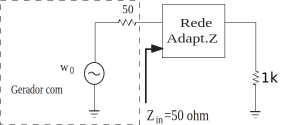
\includegraphics[scale=1]{Imagens/redeL.pdf}
    \label{fig:redeL}
    
    \small Fonte: Me. Jaime Laelson Jacob, 2016.
\end{figure}

\begin{enumerate}[label=\alph*]
    \item Montar o circuito com a rede adaptadora projetada;
    
    \item Injetar um sinal senoidal de frequência $\omega_0$ e
    amplitude da ordem de centenas de milivolts de pico na entrada do circuito montado.
    
    \item Observar a forma de onda da entrada, sobre a carga à saída e sobre a carga resistiva à saída. Anotar as formas de onda.
    
    \item Variar a frequência do sinal senoidal até obter o perfeito casamento de impedância entre fonte e carga. Anotar esta frequência.
    
    \item Obter o índice de mérito do circuito completo ($Q_{Load}$). Calcular este paramento e comparar com o medido. Obter a banda de passagem da rede adotando um dos critérios para adaptação de impedância, sintetizados nas equações (6) e (7).
   \end{enumerate} 

2- Reprojetar a rede adaptadora utilizando 3 elementos (rede T ou $\pi$). Admita agora que não há restrição para o bloqueio de eventuais componentes
DC entre fonte e carga.
\begin{enumerate}[label=\alph*]
    \item Variar a frequência do sinal senoidal até obter o perfeito casamento de impedância entre fonte e carga. Anotar esta frequência.
    
    \item  Obter, através de um procedimento experimental, o novo índice de mérito carregado para a rede de 3 elementos. Comparar com o valor teórico do projeto.
    
    \item Qual a banda de passagem para esta topologia. Adote o mesmo critério utilizado anteriormente.
\end{enumerate}


\subsubsection{Rede Adaptadora de Banda Larga (WBand)}

A partir do problema de adaptação de impedância mostrado na figura 2, calcular e implementar uma rede de banda larga de 2 seções L de tal forma a maximizar a banda de passagem. Nesta condição, calcular o índice de qualidade carregado do circuito. Como frequência central de projeto, adote a mesma do item anterior.

Passos experimentais:
\begin{enumerate}[label=\alph*]
    \item Montar o circuito com a rede adaptadora WBand projetada.
    
    \item  Obter a BW da rede adotando o mesmo critério utilizado anteriormente na obtenção da BW da rede de banda estreita. Comparar o incremento na BW com relação ao caso anterior.
    
    \item Medir o $Q_{rede}$ WBand e comparar com o valor teórico.
\end{enumerate}


\newpage
\section{Resultados}

\subsection{4-PAM com codificação binária}

Na figura \ref{fig:sinais1}, são mostrados os sinais do sistema PAM com codificação binária. Como pode-se notar na legenda observa-se os pontos onde ocorreu a leitura de sinal. Como nota-se quando comprara-se o sinal transmitido ao recebido, percebe-se um atraso de aproximadamente 6 bits.

\begin{figure}[H]
    \centering
    \includegraphics[scale=0.4]{sinalbin}
    \caption{Sinais obtidos.}
    \label{fig:sinais1}
\end{figure}

Quanto ao desempenho do sistema, a tabela \ref{tab:3} mostra a taxa de erro de bit e a probabilidade de erro em função da razão energia de bit e potência do ruído, sendo que a figura \ref{fig:bin} mostra a representação gráfica da BERx$\frac{Eb}{No}$.

\begin{small}
    \begin{table}[H]
        \begin{center}
            \caption{Tabela BER x Eb/No}
            \begin{tabular}{c|c|c}
                \hline
                $\frac{Eb}{No}$ [dB] & BER & $P_b$ \\
                \hline
                $\infty$ & 0 & 0 \\
                \hline
                10 & 0.0031  & $2.4 \times 10^{-3} $ \\
                \hline
                8 & $1.28 \times 10^{-3}$ & 0.0123 \\
                \hline
                6 & 0.0396 &  0.0372 \\
                \hline
                4 & 0.077 &  0.0782 \\
                \hline
                2 & 0.1311 & 0.1301 \\
                \hline
                0 & 0.1821 & 0.1855 \\
                \hline
            \end{tabular}
            \label{tab:3}
        \end{center}
    \end{table}
\end{small}

\begin{figure}[H]
    \centering
    \includegraphics[scale=0.4]{bin}
    \caption{BER com código binário.}
    \label{fig:bin}
\end{figure}



\subsection{4-PAM com codificação Gray}

Na figura \ref{fig:sinais2}, são mostrados os sinais do sistema PAM com codificação gray. Como pode-se notar na legenda observa-se os pontos onde ocorreu a leitura de sinal. Como nota-se quando comprara-se o sinal transmitido ao recebido, percebe-se um atraso de aproximadamente 6 bits.

\begin{figure}[H]
    \centering
    \includegraphics[scale=0.4]{sinalgray}
    \caption{Sinais obtidos.}
    \label{fig:sinais2}
\end{figure}

Quanto ao desempenho do sistema, a tabela \ref{tab:4} mostra a taxa de erro de bit e a probabilidade de erro em função da razão energia de bit e potência do ruído, sendo que a figura \ref{fig:gray} mostra a representação gráfica da BERx$\frac{Eb}{No}$.

\begin{small}
    \begin{table}[H]
        \begin{center}
            \caption{Tabela BER x Eb/No}
            \begin{tabular}{c|c|c}
                \hline
                $\frac{Eb}{No}$ [dB] & BER & $P_b$ \\
                \hline
                $\infty$ & 0 & 0 \\
                \hline
                10 & 0.0019 & $1.8 \times 10^{-3} $ \\
                \hline
                8 & $8.6 \times 10^{-3}$ & 0.0092 \\
                \hline
                6 & 0.0274 &  0.0279 \\
                \hline
                4 & 0.0595 & 0.0586 \\
                \hline
                2 & 0.0954 & 0.0976 \\
                \hline
                0 & 0.1463 & 0.1392 \\
                \hline
            \end{tabular}
            \label{tab:4}
        \end{center}
    \end{table}
\end{small}

\begin{figure}[H]
    \centering
    \includegraphics[scale=0.4]{gray}
    \caption{BER com código Gray.}
    \label{fig:gray}
\end{figure}


Para finalizar, a figura \ref{fig:bxg} mostra o gráfico de desempenho para as duas codificações, onde nota-se claramente a vantagem da codificação gray em relação a codificação binária.

\begin{figure}[H]
    \centering
    \includegraphics[scale=0.4]{bxg}
    \caption{Exemplo de figura}
    \label{fig:bxg}
\end{figure}
\newpage
\section{Discussão e Conclusão}
As simulações tiveram resultados condizentes com a teoria, comprovando na prática, diversos circuitos relacionados com esse relatório sobre modulações ASK, PSK e FSK. É super interessante observar essas modulações na prática para ter convicção e compreensão de seus funcionamentos. As primeiras imagens de cada item na parte experimental provam todos esses funcionamentos.
Sobre a BER, observa-se um valor bastante próximo entre teoria e prática, gerando maior confiabilidade nos sistemas na hora de implementação dentro de um circuito, porém na última imagem (41) é onde encontra-se o maior resultado, onde compara-se todas as 3 modulações e verifica-se que a modulação PSK possui uma atenuação muito menor se comparado com os outros tipos de modulação, não que as outras sejam ruins, porém a PSK é um método que consegue garantir garantia do sinal próximo de íntegro de uma transmissão no meio de telecomunicações.
\newpage

\nocite{*}
\bibliography{config}{}
\bibliographystyle{ieeetr}
\end{document}